\section {Oscillation fit to the $3.23\times10^{19}$ POT dataset}
\label{sec:oscfit_runI}

Using the method outlined in the previous sections,
an oscillation fit was performed to the 2010a $3.23\times10^{19}$ POT dataset.
For GENIE, this analysis finds
$|\Delta m^{2}_{23}|$ = 2.8$\times$10$^{-3}$ $eV^{2}/c^{4}$ and
$sin^{2}2\theta_{23}$ = 0.81
as the best-fit values.
For NEUT, the corresponding values are
$|\Delta m^{2}_{23}|$ = 2.9$\times$10$^{-3}$ $eV^{2}/c^{4}$ and
$sin^{2}2\theta_{23}$ = 0.83.
The reconstructed neutrino energy distribution for the 8 1-ring $\mu$-like events of the 
2010a dataset, along with the best-fit predictions from GENIE and NEUT are shown in  
Figs. \ref{fig:fit2010a_spectrum_and_data_genie} and \ref{fig:fit2010a_spectrum_and_data_neut}.

The systematic errors at the best-fit point were evaluated as described in 
Sec. \ref{sec:systematics_at_osc_bestfit}.
The systematic errors at the GENIE best-fit point are given, 
in Tab. \ref{table:oscsyst_at_genie_bestfit_point}. 
For NEUT, the systematic errors at the best-fit point
are given in Tab. \ref{table:oscsyst_at_neut_bestfit_point}.
We list the effect on $|\Delta m^{2}_{23}|$ and $sin^{2}2\theta_{23}$ of
all systematic uncertainties considered in this analysis.
The total systematic error is computed by adding 
in quadrature
the errors due to individual systematic uncertainties.
This analysis finds that the combined systematic uncertainty at the GENIE (NEUT) best-fit point 
is 4.3\% (3.9\%) for $|\Delta m^{2}_{23}|$ and 6.7\% (6.0\%) for $sin^{2}2\theta_{23}$.
The SuperK NC efficiency, the CCQE cross section and the flux shape uncertainties 
are the ones with the largest impact on $|\Delta m^{2}_{23}|$.
The dominant systematics on $sin^{2}2\theta_{23}$ are the SuperK CCQE efficiency,
the flux normalization, the ND280 efficiency and the CCother/CCQE cross section ratio.

Confidence regions were calculated using both methods described in Sec. \ref{sec:contours}.
A comparison of the Feldman-Cousins and plain confidence regions (including statistical errors only) 
for the 2010a dataset is shown in Fig. \ref{fig:fit2010a_compare_fc_nonfc_statonly}.
As discussed in Sec. \ref{sec:contours} the Feldman-Cousins confidence regions have correct coverage 
by construction. 
As it can be seen in Fig. \ref{fig:fit2010a_compare_fc_nonfc_statonly},
the Feldman-Cousins and plain confidence regions differ significantly
and, therefore, the coverage of the latter is spurious.
The plain confidence regions tend to overcover near a physical boundary, and either
undercover or overcover away from that boundary. 
Consequently, this analysis considers only the Feldman-Cousins method for quoting
the final results.
The 68\%, 90\% and 95\% Feldman-Cousins confidence regions, with and without systematics, for the 2010a
$\nu_{\mu}$ disappearance analysis are shown in
Fig. \ref{fig:fit2010a_confregion_genie} for GENIE and in
Fig. \ref{fig:fit2010a_confregion_neut} for NEUT.
The estimated systematic error at the best-fit point 
(listed in Tabs. \ref{table:oscsyst_at_genie_bestfit_point} and \ref{table:oscsyst_at_neut_bestfit_point})
is also shown.

Upon seeing the reconstructed energy distribution of the 2010a dataset, it was clear to the authors
of this note that large values of $|\Delta m^{2}_{23}|$, in the wrong trough of the oscillation survival
probability function, may provide a better fit to the data.
The oscillation parameter limits (discussed in Sec. \ref{sec:osc_par_limits}) were relaxed and a new fit
was performed. The result is shown in Fig. \ref{fig:fit2010a_wide_dmsq_genie}.
Indeed, a better fit to the data exists at maximal mixing angle and
large $|\Delta m^{2}_{23}|$ (of the order of 10$^{-2}$ eV$^{2}$/c$^{4}$,
some $\sim$ 20$\sigma$ away from the MINOS best-fit value).
As it can be seen in Fig. \ref{fig:fit2010a_wide_dmsq_genie},
much of the $\chi^{2}$ valley at large $|\Delta m^{2}_{23}|$, is lower than the
best-fit point in the 
$|\Delta m^{2}_{23}|$ window
from 10$^{-3}$ eV$^{2}$/c$^{4}$ to 6$\times$10$^{-3}$ eV$^{2}$/c$^{4}$.
Fig. \ref{fig:fit2010a_wide_dmsq_marginalised_genie} shows 
the marginalised $\chi^{2}$ distributions from the fit shown in Fig. \ref{fig:fit2010a_wide_dmsq_genie}.

Although the high $|\Delta m^{2}_{23}|$ solution was pointed-out by the authors of this analysis,
the majority of the authors feel uneasy modifying the pre-defined analysis procedure 
after seeing the actual data (in response to a statistical fluctuation in the observed dataset).
The pre-defined $|\Delta m^{2}_{23}|$ limits of 1$\times$10$^{-3}$ eV$^{2}$/c$^{4}$ and 6$\times$10$^{-3}$ eV$^{2}$/c$^{4}$
correspond to the T2K sensitivity window, as it can be seen clearly in Fig. \ref{fig:sk_spectrum_sensitivity_limits_and_highDm2}.
The limits were set (before looking at the data) exactly so as to avoid fluctuations such as the one observed in the data.
This entire experiment (and analysis) was built on the premise that the first oscillation minimum is around the T2K peak energy,
as was determined by MINOS and K2K. 
In addition, including this prior knowledge (Bayesian prior) into the oscillation result does
not invalidate the frequentist interpretation of the confidence regions as it has been incorrectly indicated \cite{Mauro}.
The SuperK expectation already employs a host of other Bayesian priors;
they are physics parameters, such as the quasi-elastic axial mass, which are selected based on belief from
(sometimes) conflicting experimental results.
Still, one can certainly assert that the 68\% confidence regions shown in this analysis is the region where 68\% of the 
measurements would fall if the same measurement could be repeated N times. 
The statement implies analysing N independent 3.23E+19 POT datasets using the exact same input assumptions (Bayesian priors).
The confidence regions shown here have correct coverage and proper frequestist interpretation 
in the $|\Delta m^{2}_{23}|$ window
from 10$^{-3}$ eV$^{2}$/c$^{4}$ to 6$\times$10$^{-3}$ eV$^{2}$/c$^{4}$.
The arguments against showing confidence regions from a fit to an enlarged $|\Delta m^{2}_{23}|$ range were made 
convincingly in \cite{DeanAndNick} and will not be repeated here. 
For the actual publication it is proposed that 
a) we show the best-fit value and confidence regions in the restricted $|\Delta m^{2}_{23}|$ range, and 
b) we indicate the existence of a global minimum outside the restricted $|\Delta m^{2}_{23}|$ range
   and we quote the probability for such a fluctuation.
The probability for such a $|\Delta m^{2}_{23}|$ fluctuation with a $3.23\times10^{19}$ POT exposure is
about 5.6\% (see Fig. \ref{fig:dmsq-distribution-2p35Em3-1p0-1x}). With $1\times10^{20}$ POT (dataset already accumulated at the time of revisiting
this note) the probability for such a fluctuation has already fallen to about 0.2\% (see Fig. \ref{fig:dmsq-distribution-2p35Em3-1p0-3x}).

\begin{table*}[htb]
\center
\renewcommand{\arraystretch}{1.75} % enlarge line spacing
\begin{tabular}{|c|cc|}
\hline
Error source  &
  $\Big(\frac{\delta{\Delta m^{2}_{23}}}{\Delta m^{2}_{23}}\Big)$  & $\Big(\frac{\delta{\sin^{2}2\theta_{23}}}{sin^{2}2\theta_{23}}\Big)$  \\
\hline
SuperK CCQE efficiency            &   0.5\%   &   2.9\%      \\
SuperK CCnonQE efficiency         &   1.0\%   &   1.6\%      \\
SuperK NC efficiency              &   2.0\%   &   1.8\%      \\
SuperK $\nu_{e}$ CC efficiency    &   0.0\%   &   0.0\%      \\
SuperK energy scale               &   0.5\%   &   0.3\%      \\
ND280 efficiency                  &   0.2\%   &   2.2\%      \\
Flux normalization                &   0.3\%   &   2.8\%      \\
Flux shape                        &   2.6\%   &   1.0\%      \\
CCQE cross section                &   1.8\%   &   1.8\%      \\
CC1pi/CCQE cross section ratio    &   1.1\%   &   1.1\%      \\
CCother/CCQE cross section ratio  &   0.4\%   &   2.6\%      \\
NC/CCQE cross section ratio       &   0.5\%   &   0.1\%      \\
FSI                               &   0.2\%   &   1.1\%      \\
\hline
Total                             &   4.3\%   &   6.7\%      \\
\hline
\end{tabular}\\[2pt]
\caption{
  Oscillation systematics computed using GENIE, at the GENIE best-fit point
  ($sin^{2}2\theta_{23}$ = 0.81 and $\Delta m^{2}_{23}$ = 2.8$\times10^{-3}$ $eV^{2}/c^{4}$).
}
\label{table:oscsyst_at_genie_bestfit_point}
\end{table*}


\begin{table*}[htb]
\center
\renewcommand{\arraystretch}{1.75} % enlarge line spacing
\begin{tabular}{|c|cc|}
\hline
Error source  &
  $\Big(\frac{\delta{\Delta m^{2}_{23}}}{\Delta m^{2}_{23}}\Big)$  & $\Big(\frac{\delta{\sin^{2}2\theta_{23}}}{sin^{2}2\theta_{23}}\Big)$  \\
\hline
SuperK CCQE efficiency            &   0.6\%   &   2.6\%      \\
SuperK CCnonQE efficiency         &   1.0\%   &   1.7\%      \\
SuperK NC efficiency              &   1.6\%   &   1.5\%      \\
SuperK $\nu_{e}$ CC efficiency    &   0.0\%   &   0.0\%      \\
SuperK energy scale               &   0.5\%   &   0.4\%      \\
ND280 efficiency                  &   0.2\%   &   2.1\%      \\
Flux normalization                &   0.3\%   &   2.6\%      \\
Flux shape                        &   2.3\%   &   1.1\%      \\
CCQE cross section                &   1.7\%   &   1.4\%      \\
CC1pi/CCQE cross section ratio    &   1.0\%   &   0.8\%      \\
CCother/CCQE cross section ratio  &   0.5\%   &   2.1\%      \\
NC/CCQE cross section ratio       &   0.4\%   &   0.1\%      \\
FSI                               &   0.4\%   &   1.1\%      \\
\hline
Total                             &   3.9\%   &   6.0\%      \\
\hline
\end{tabular}\\[2pt]
\caption{
  Oscillation systematics computed using NEUT, at the NEUT best-fit point
  ($sin^{2}2\theta_{23}$ = 0.83 and $\Delta m^{2}_{23}$ = 2.9$\times10^{-3}$ $eV^{2}/c^{4}$).
}
\label{table:oscsyst_at_neut_bestfit_point}
\end{table*}



\begin{figure*}[htb]
\center
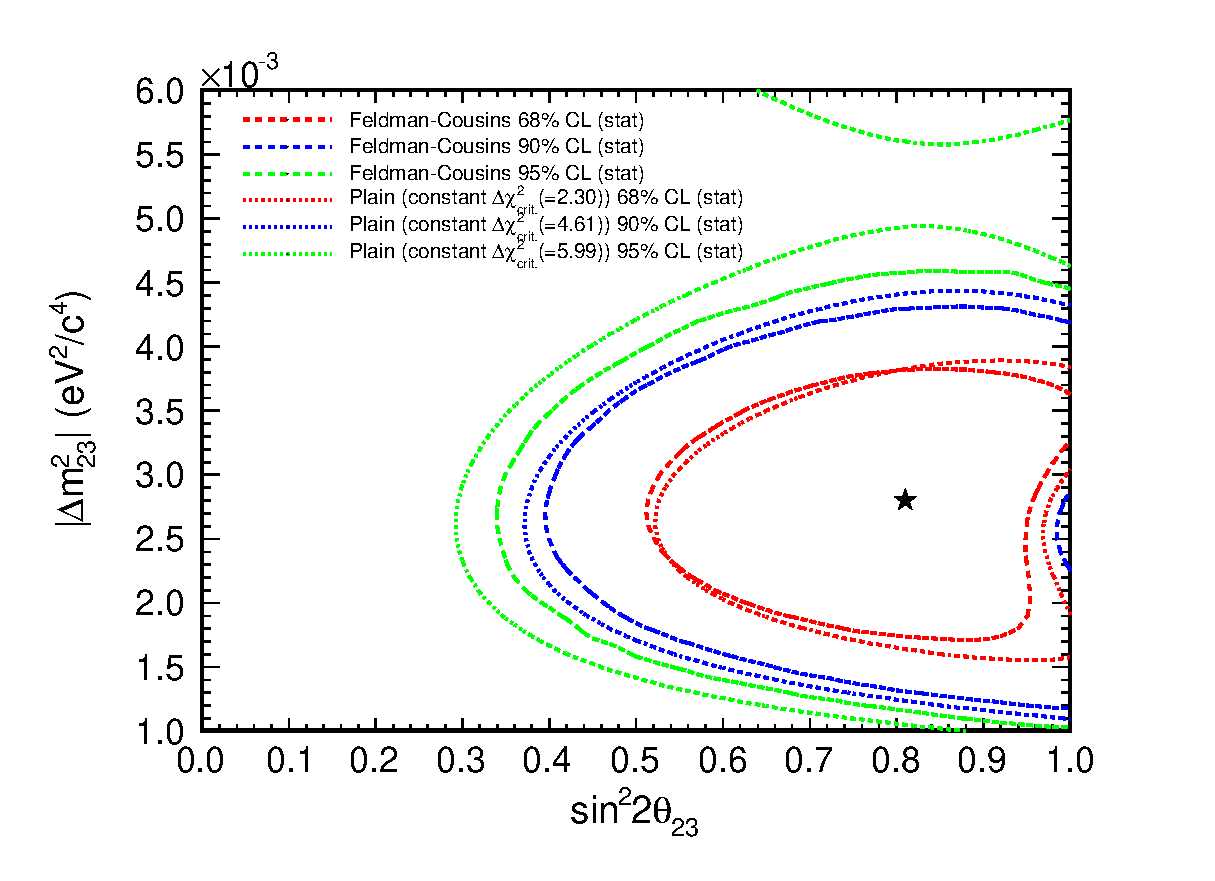
\includegraphics[width=42pc]{./images/fits/2010a/contour_stat_genie_compare_fc_nonfc.eps}
\caption{
 Comparison of the Feldman-Cousins and plain confidence regions (including statistical errors only)
 for the 2010a dataset. As discussed in Sec. \ref{sec:contours} the Feldman-Cousins confidence regions 
 have correct coverage by construction. 
 The Feldman-Cousins and plain confidence regions differ significantly and, therefore,
 coverage of the plain contours is spurious. The latter seem to overcover significantly
 near the physical boundary and undercover away from it.
 In addition, the non plain contour appears to ignore the existence of $\Delta m^{2}_{23}$ boundaries
 (fitter limits). 
 The contours are shown for GENIE.
 Identical conclusions are drawn by the comparison of the Feldman-Cousins and plain confidence regions 
 generated by NEUT.
}
\label{fig:fit2010a_compare_fc_nonfc_statonly}
\end{figure*}

\begin{figure*}[htb]
\center
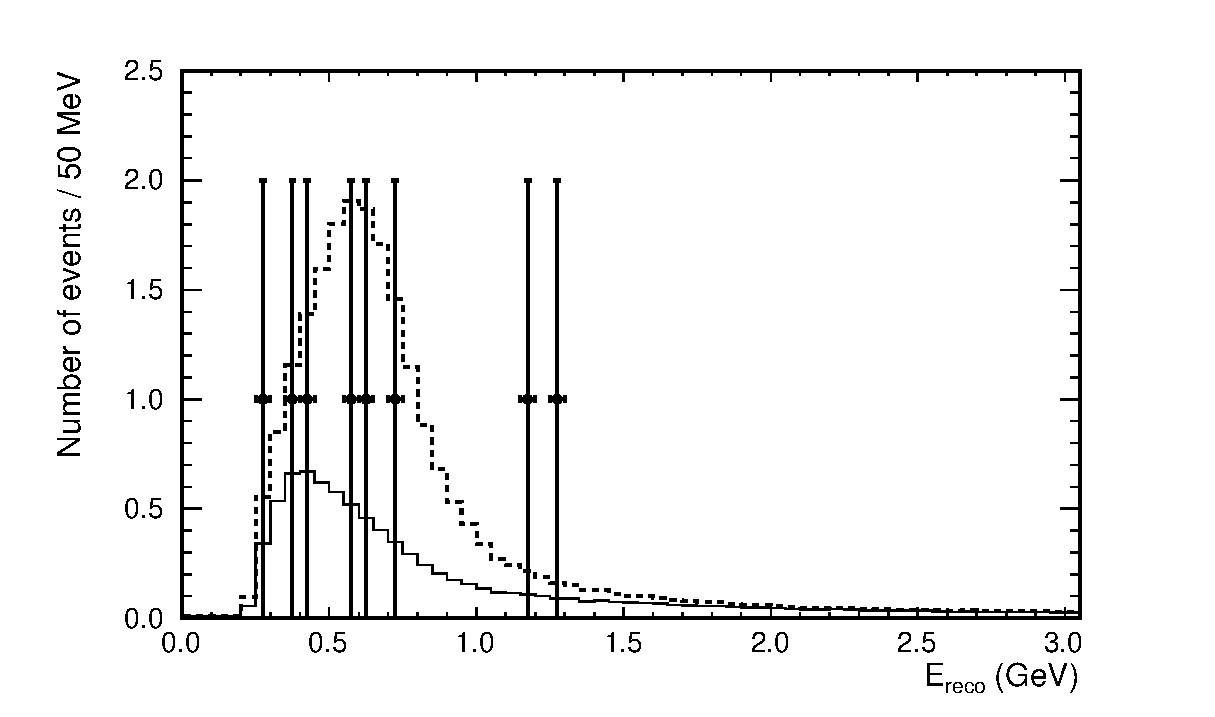
\includegraphics[width=28pc]{./images/fits/2010a/genie_bestfit_spectrum.eps}
\caption{
  Reconstructed neutrino energy distribution for the 8 1-ring $\mu$-like events of the 
  2010a 3.23$\times$10$^{19}$ POT dataset (points) and GENIE best-fit SuperK prediction (solid line).
  The best-fit oscillation parameters (in the search window defined in Sec. \ref{sec:osc_par_limits}) are 
  $|\Delta m^{2}_{23}|$ = 2.8$\times$10$^{-3}$ $eV^{2}/c^{4}$ and $sin^{2}2\theta_{23}$ = 0.81.
  The dotted line shows the GENIE prediction without oscillations.
}
\label{fig:fit2010a_spectrum_and_data_genie}
\end{figure*}

\begin{figure*}[htb]
\center
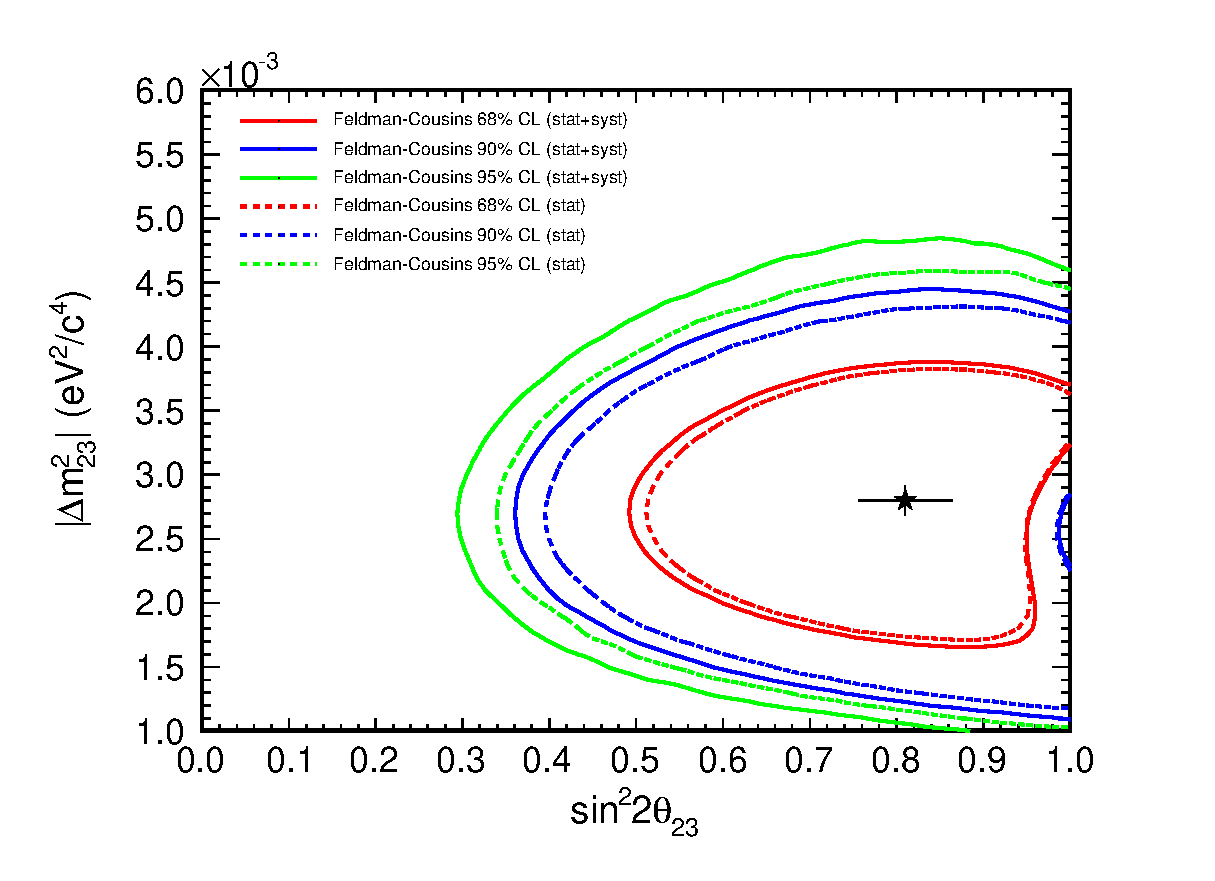
\includegraphics[width=36pc]{./images/fits/2010a/contour_statsyst_andbestfitsyst_genie.eps}
\caption{
  68\%, 90\% and 95\% Feldman-Cousins confidence regions, with and without systematics,
  for the GENIE disappearance fit to the 2010a dataset.
  The estimated systematic error at the best-fit point is also shown with a cross.
}
\label{fig:fit2010a_confregion_genie}
\end{figure*}

\begin{figure*}[htb]
\center
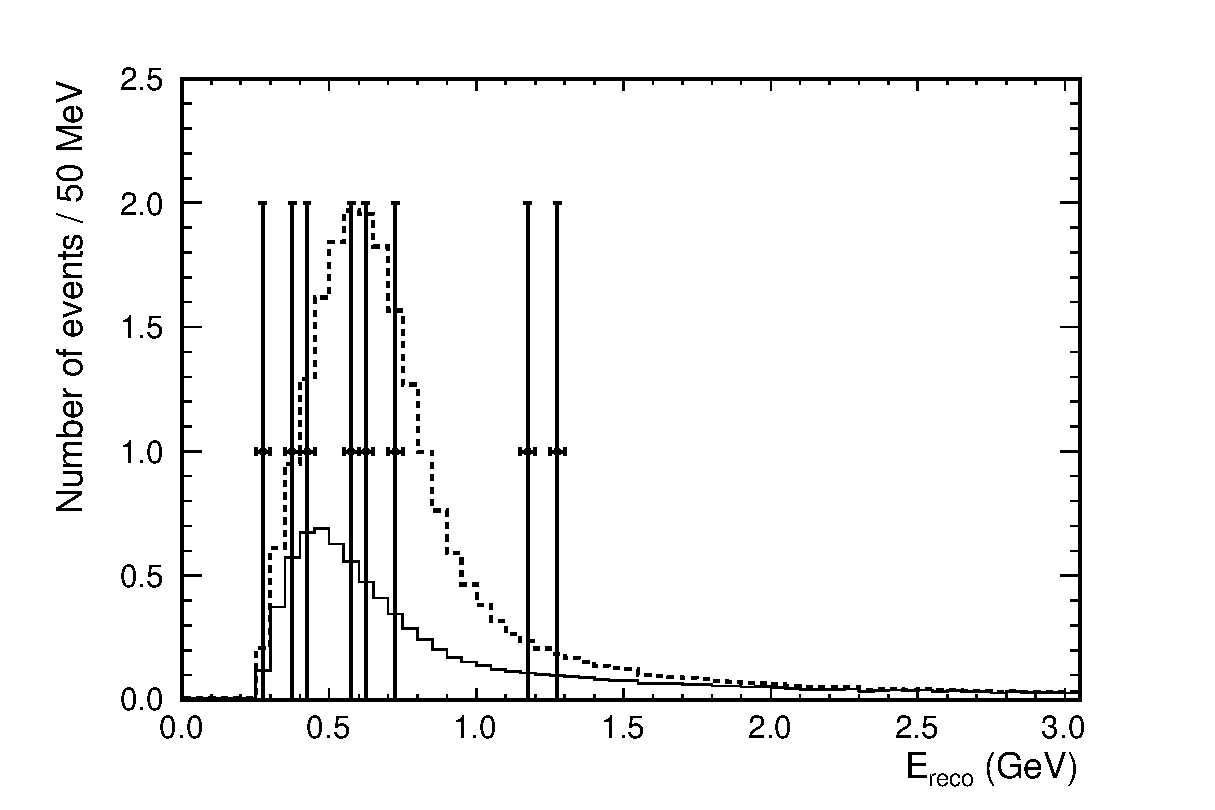
\includegraphics[width=28pc]{./images/fits/2010a/neut_bestfit_spectrum.eps}
\caption{
  Reconstructed neutrino energy distribution for the 8 1-ring $\mu$-like events of the 
  2010a 3.23$\times$10$^{19}$ POT dataset (points) and NEUT best-fit SuperK prediction (solid line).
  The best-fit oscillation parameters (in the search window defined in Sec. \ref{sec:osc_par_limits}) are 
  $|\Delta m^{2}_{23}|$ = 2.9$\times$10$^{-3}$ $eV^{2}/c^{4}$ and $sin^{2}2\theta_{23}$ = 0.83.
  The dotted line shows the NEUT prediction without oscillations.
}
\label{fig:fit2010a_spectrum_and_data_neut}
\end{figure*}

\begin{figure*}[htb]
\center
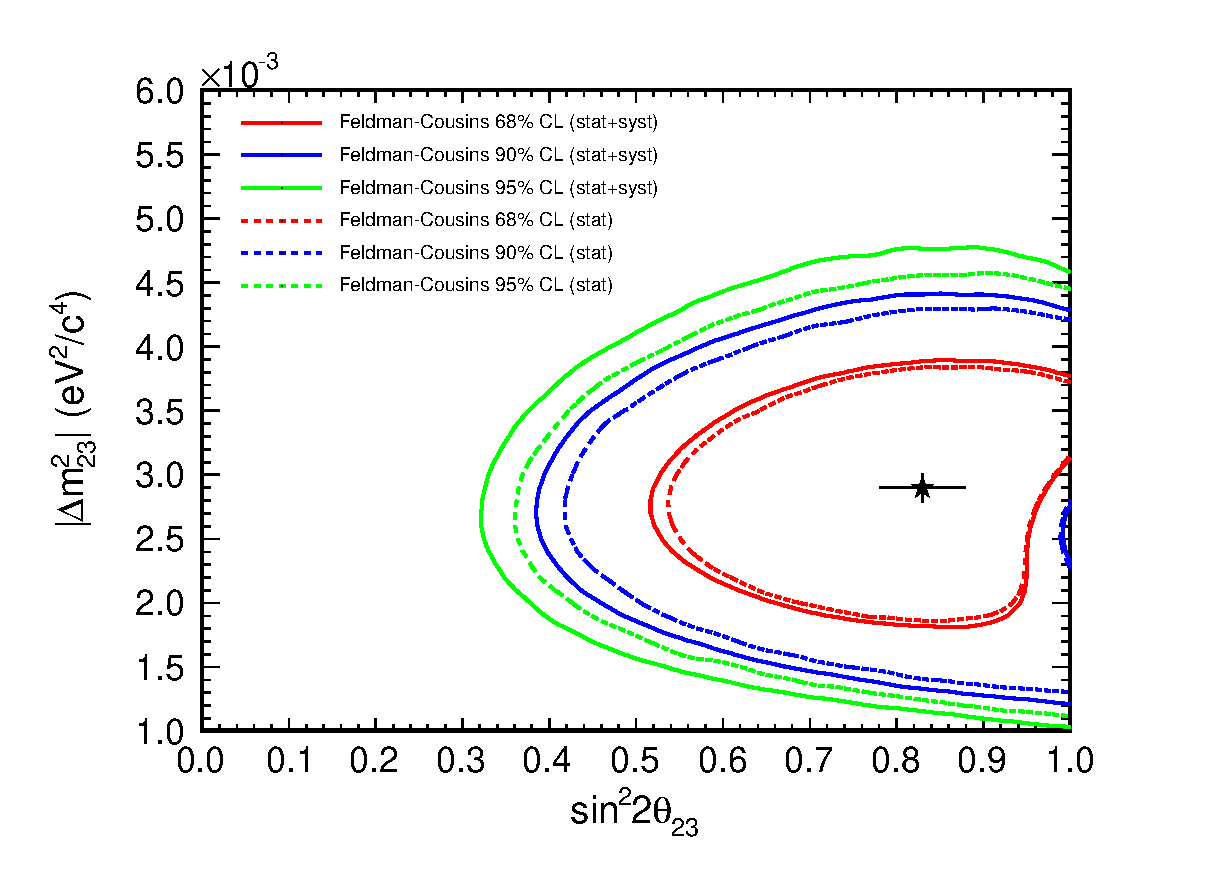
\includegraphics[width=36pc]{./images/fits/2010a/contour_statsyst_andbestfitsyst_neut.eps}
\caption{
  68\%, 90\% and 95\% Feldman-Cousins confidence regions, with and without systematics,
  for the NEUT disappearance fit to the 2010a dataset.
  The estimated systematic error at the best-fit point is also shown with a cross.
}
\label{fig:fit2010a_confregion_neut}
\end{figure*}


\begin{figure*}[htb]
\center
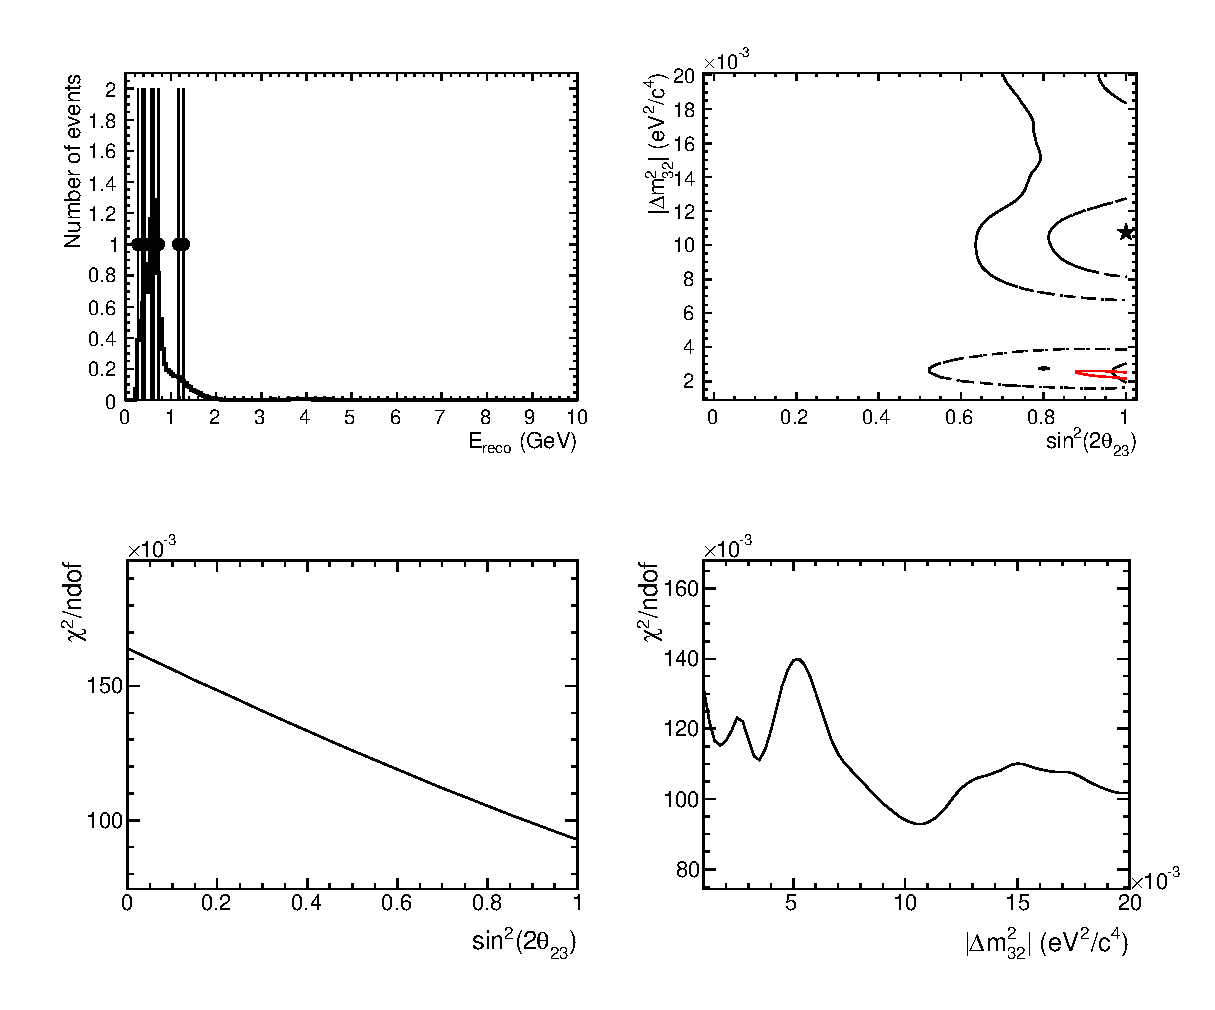
\includegraphics[width=28pc]{./images/fits/2010a/fit_2010a_genie_wide.eps}
\caption{
  Fit to the 2010a set with relaxed upper limit of $|\Delta m^{2}_{23}|$.
  The top-left plot shows the reconstructed energies of the 2010a dataset and the best-fit prediction.
  The confidence regions shown on the top-right are the 68\% and 90\% CL regions (statistical errors only) 
  calculated, for simplicity, using the PDG method.
  For reference, the MINOS 90\% CL region is also shown (red line).
  The best-fit point is shown with a black-star.
  The bottom-left and bottom-right plots show the $\chi^{2}$/ndof along the $sin^{2}2\theta_{23}$ and $|\Delta m^{2}_{23}|$
  lines that pass through the best-fit point.
}.
\label{fig:fit2010a_wide_dmsq_genie}
\end{figure*}

\begin{figure*}[htb]
\center
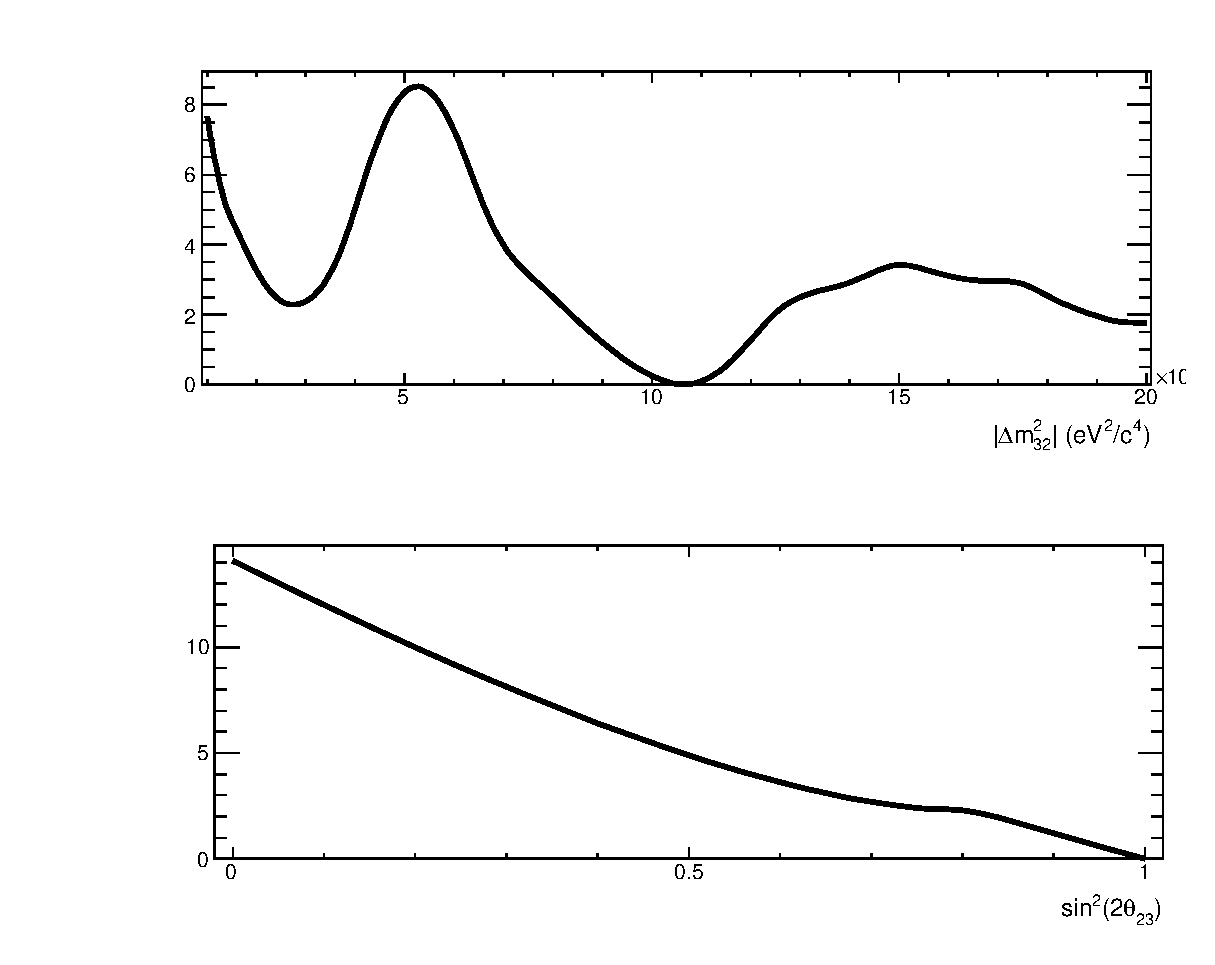
\includegraphics[width=24pc]{./images/fits/2010a/fit_2010a_genie_wide_marginalised_chisq.eps}
\caption{
  Marginalised $\chi^{2}$ distributions for the fit shown in Fig. \ref{fig:fit2010a_wide_dmsq_genie}.
}
\label{fig:fit2010a_wide_dmsq_marginalised_genie}
\end{figure*}


\begin{figure*}[htb]
\center
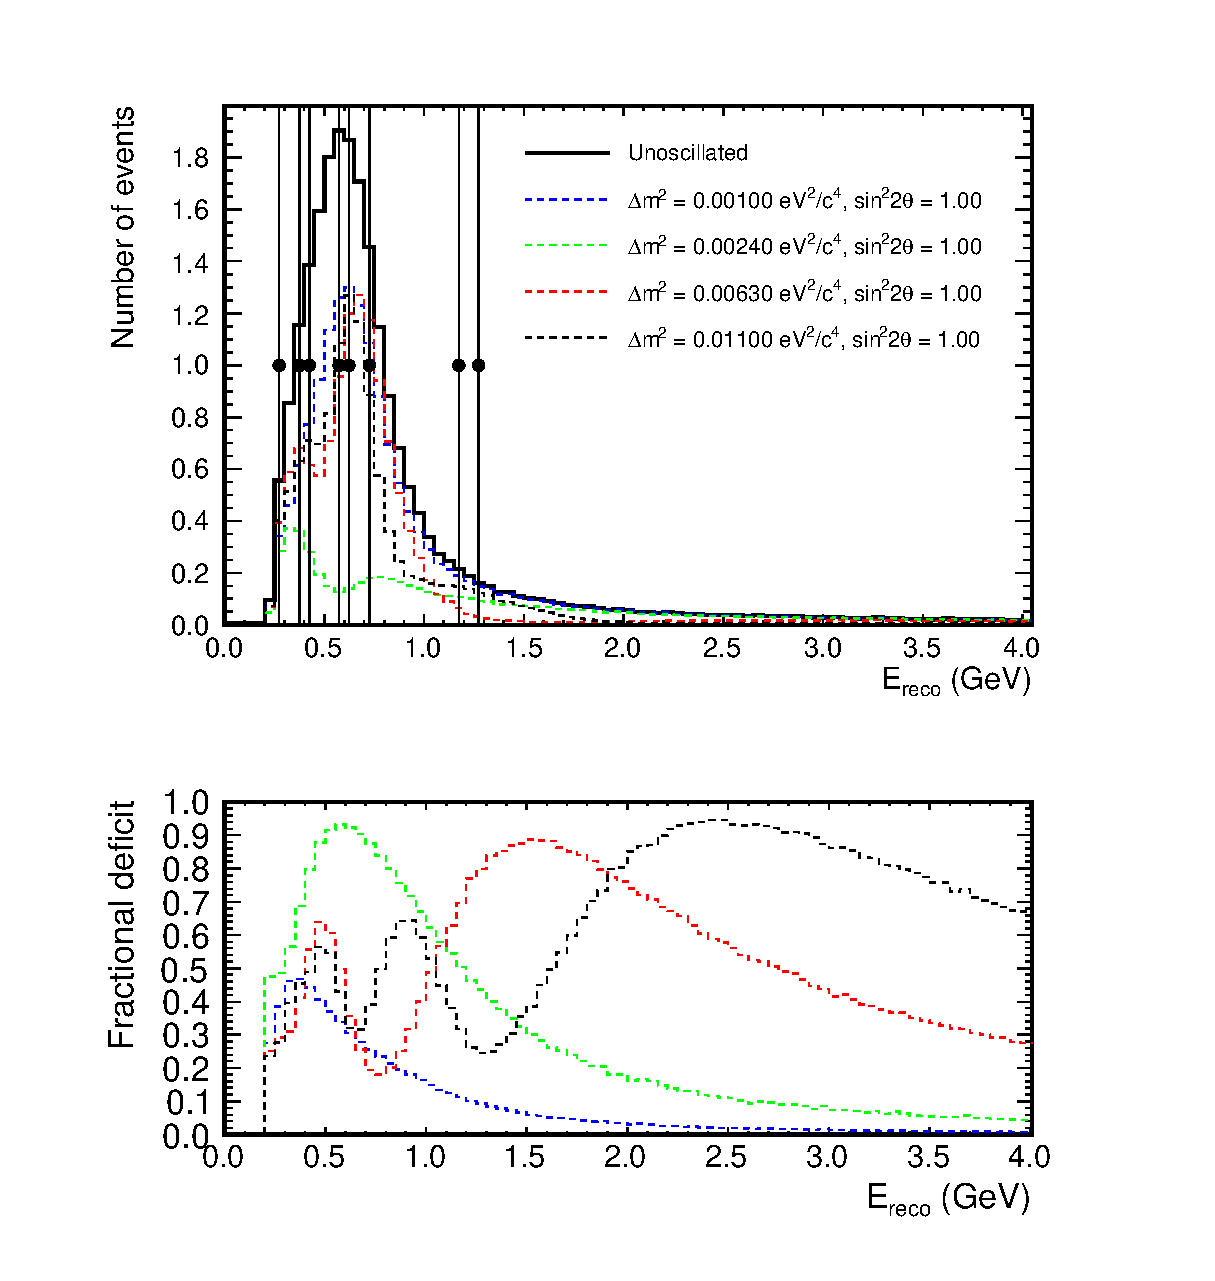
\includegraphics[width=38pc]{./images/etc/sk_spectrum_sensitivity_limits_and_highDm2_data.eps}
\caption{
  Predicted reconstructed-energy spectrum of 1-ring $\mu$-like events (after extrapolation)
  for $sin^{2}2\theta_{23}$ = 1.0 and
  $\Delta m^{2}_{23}$ =
    1.0$\times10^{-3}$ $eV^{2}/c^{4}$,
    2.4$\times10^{-3}$ $eV^{2}/c^{4}$,
    6.0$\times10^{-3}$ $eV^{2}/c^{4}$ and
    1.1$\times10^{-2}$ $eV^{2}/c^{4}$.
  The non-oscillated spectrum (GENIE) and the 2010a dataset are also shown.
  With $|\Delta m^{2}_{23}|$ = 1$\times$10$^{-3}$ eV$^{2}$/c$^{4}$ the first oscillation minimum is in the region dominated by
  NC and non-CCQE interactions. On the other hand, with $|\Delta m^{2}_{23}|$ = 6$\times$10$^{-3}$ eV$^{2}$/c$^{4}$ the (first) 
  oscillation minimum is already well above the T2K peak energy. In both of these cases, our $|\Delta m^{2}_{23}|$ messurement 
  capabilities are much deteriorated. With $\Delta m^{2}_{23}$=1.1$\times10^{-2}$ $eV^{2}/c^{4}$, the first oscillation minimum 
  appears at 2.5 GeV! The high-$\Delta m^{2}_{23}$ solution provides a better fit to the small 2010a dataset only because the 
  second and third oscillation minina happen to be accomodated between gaps (pseudo-dips) left by the 8 observed events at
  around 0.5 GeV and 1 GeV. The probability for such a $\Delta m^{2}_{23}$ fluctuation is given in the text.
}
\label{fig:sk_spectrum_sensitivity_limits_and_highDm2}
\end{figure*}

\begin{figure*}[htb]
\center
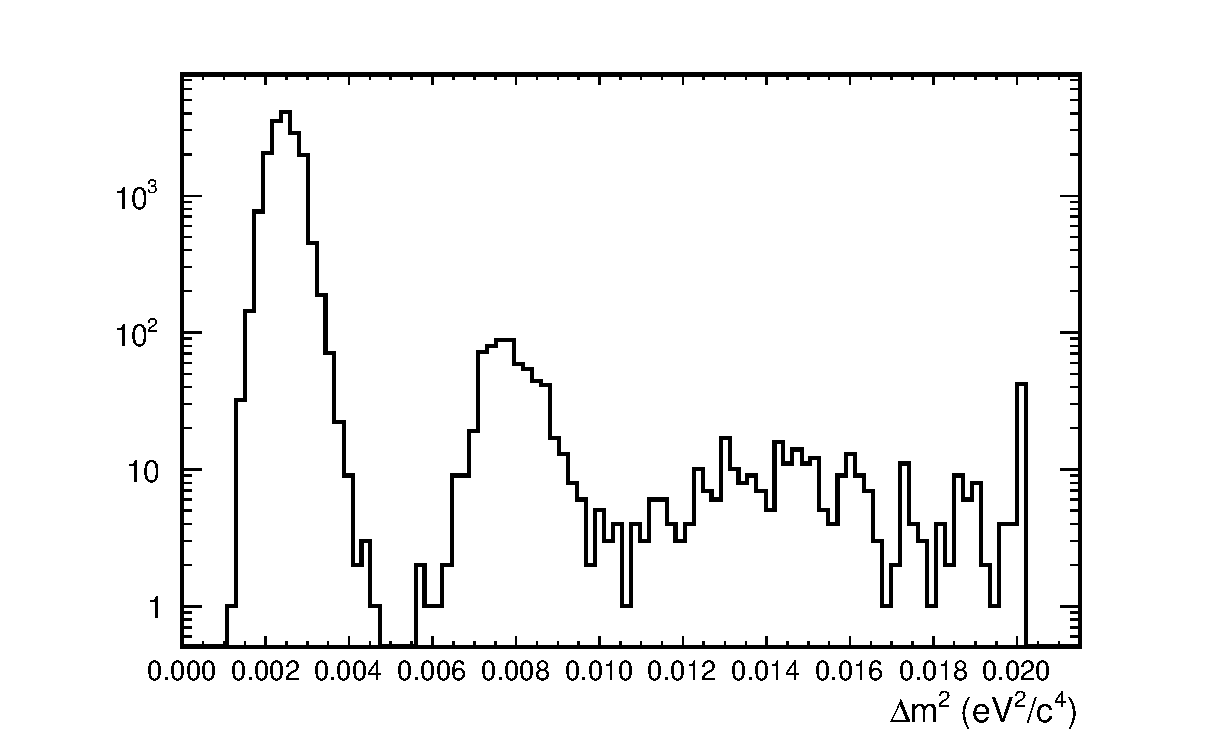
\includegraphics[width=27pc]{./images/etc/dmsq-distribution-2p35Em3-1p0-1x.eps}
\caption{
  Distribution of best-fit $\Delta m^{2}_{23}$ values for a set of toy MC experiments
  generated with the MINOS best-fit values ($\Delta m^{2}_{23}$ = 2.35$\times10^{-3}$ $eV^{2}/c^{4}$
  and maximal mixing). The toy MC experiments were generated for an 
  integrated neutrino beam exposure of $3.23\times10^{19}$ POT and systematic variations were included.
  5.6\% of fits gave a $\Delta m^{2}_{23}$ value above 6$\times10^{-3}$ $eV^{2}/c^{4}$.
}
\label{fig:dmsq-distribution-2p35Em3-1p0-1x}
\end{figure*}

\begin{figure*}[htb]
\center
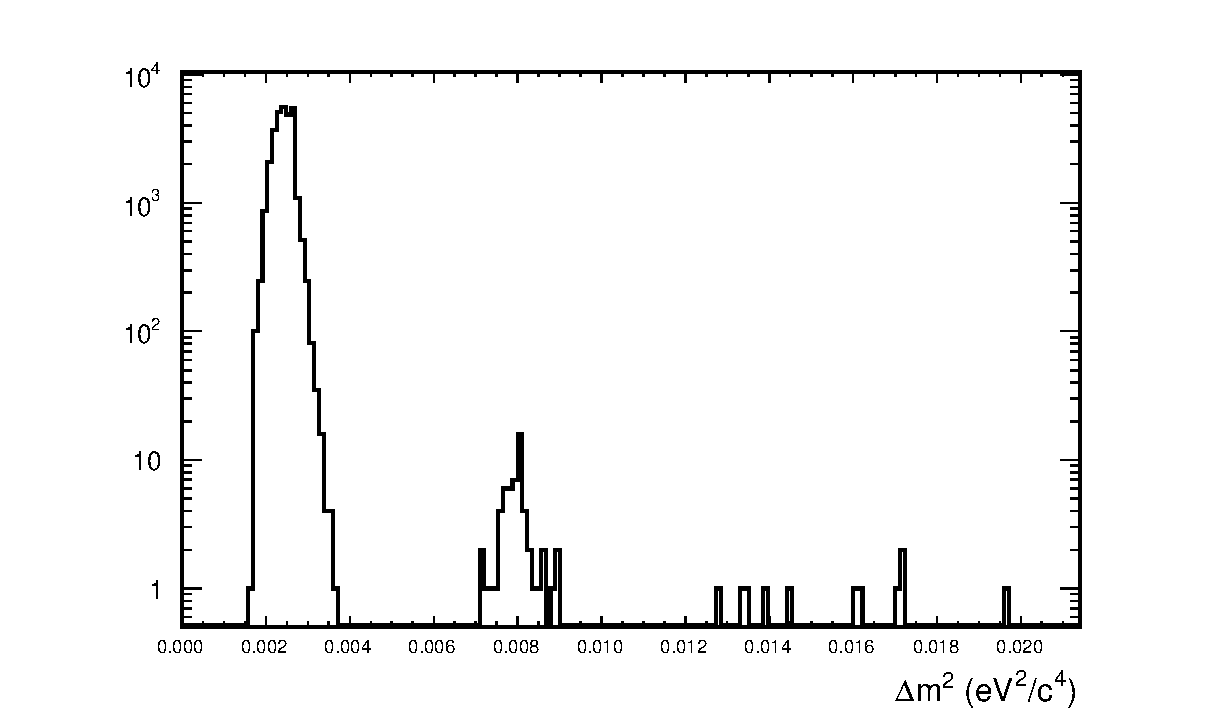
\includegraphics[width=27pc]{./images/etc/dmsq-distribution-2p35Em3-1p0-3x.eps}
\caption{
  Distribution of best-fit $\Delta m^{2}_{23}$ values for a set of toy MC experiments
  generated with the MINOS best-fit values ($\Delta m^{2}_{23}$ = 2.35$\times10^{-3}$ $eV^{2}/c^{4}$
  and maximal mixing). The toy MC experiments were generated for an 
  integrated neutrino beam exposure of $1\times10^{20}$ POT (3 $\times$ 2010a) and systematic variations were included.
  0.2\% of fits gave a $\Delta m^{2}_{23}$ value above 6$\times10^{-3}$ $eV^{2}/c^{4}$.
}
\label{fig:dmsq-distribution-2p35Em3-1p0-3x}
\end{figure*}


%
%
%\section {Alternative hypotheses fits to the $3.23\times10^{19}$ POT dataset}
%\label{sec:altfit_runI}
%
%To be written.
%
%\begin{figure*}[htb]
%\center
%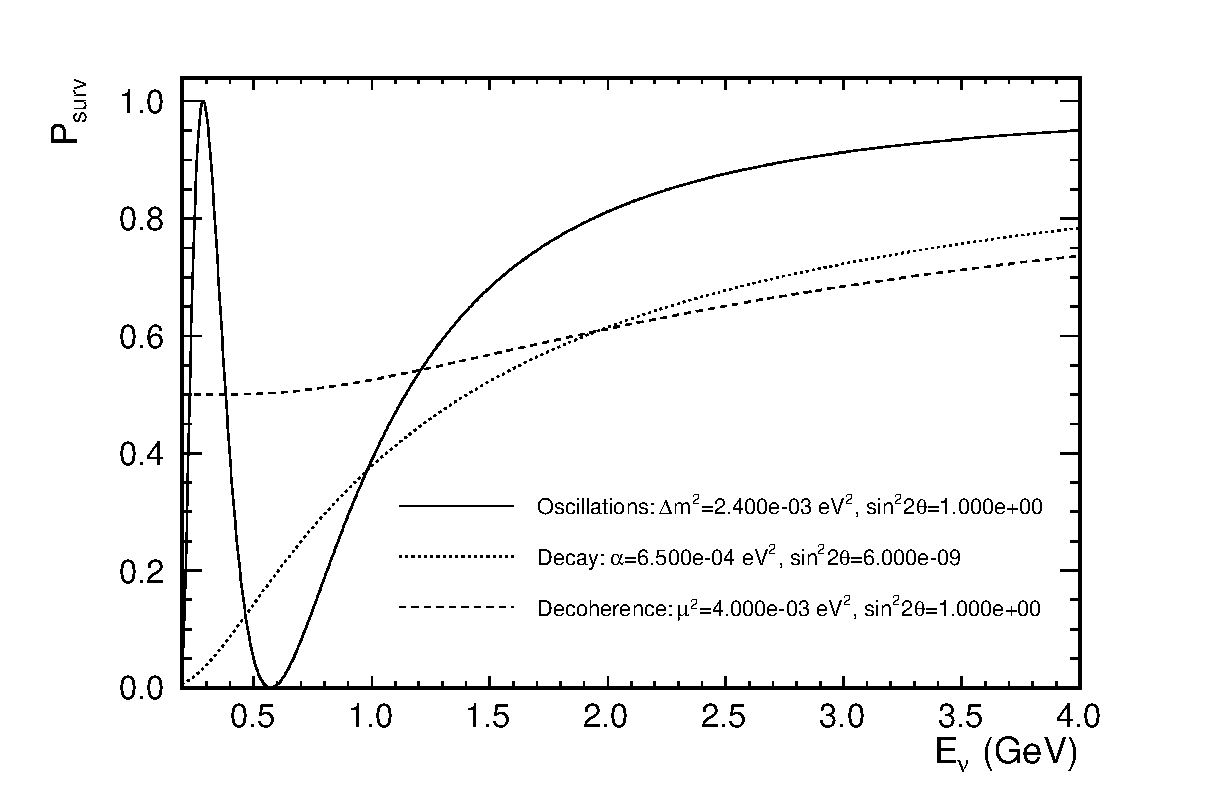
\includegraphics[width=38pc]{./images/etc/psurv_models.eps}
%\caption{
%  Estimated $\nu_{\mu}$ survival probabilities as function of true neutrino energy,
%  under the neutrino oscillation, decay \cite{Decay} and decoherence \cite{Decoherence} hypotheses.
%  Characteristic physics parameters (shown on the plot) were used for each model.
%}
%\label{fig:psurv_models}
%\end{figure*}
%
%
